% Complete set of TikZ diagrams for PhD thesis on Ontology-Driven Code Generation
% Author: Generated for ggen framework thesis
% Date: 2026-01-06
%
% This file contains all 5 architectural diagrams ready for inclusion in thesis.tex
% Each diagram is self-contained and can be compiled independently or included via \input{}
%
% Usage in main thesis:
%   \begin{figure}[h]
\centering
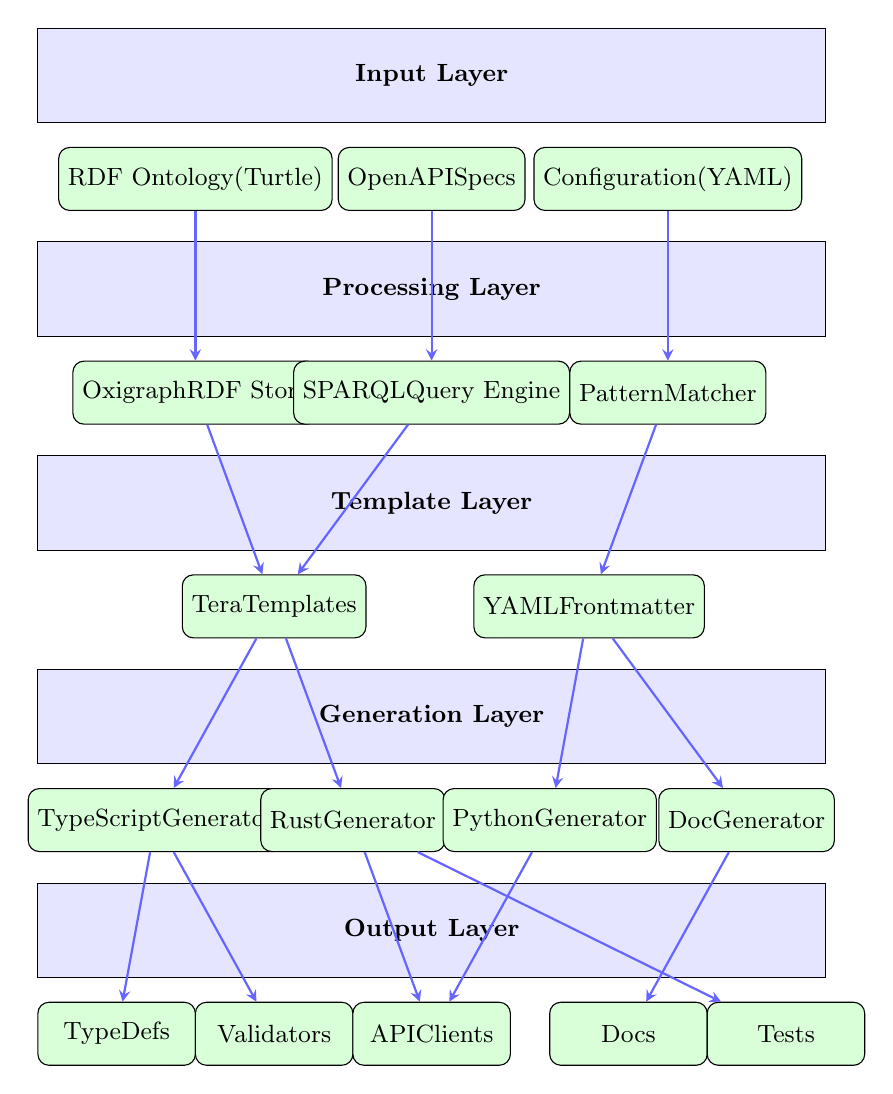
\begin{tikzpicture}[
    layer/.style={rectangle, draw, fill=blue!10, minimum width=10cm, minimum height=1.2cm, font=\small\bfseries},
    component/.style={rectangle, draw, fill=green!15, rounded corners, minimum width=2cm, minimum height=0.8cm, font=\small},
    arrow/.style={->, >=stealth, thick, color=blue!60},
    node distance=0.3cm
]

% Layer 1: Input Layer
\node[layer] (input) at (0,0) {Input Layer};
\node[component, below=of input, xshift=-3cm] (rdf) {RDF Ontology\\(Turtle)};
\node[component, below=of input] (openapi) {OpenAPI\\Specs};
\node[component, below=of input, xshift=3cm] (config) {Configuration\\(YAML)};

% Layer 2: Processing Layer
\node[layer, below=1.5cm of input] (processing) {Processing Layer};
\node[component, below=of processing, xshift=-3cm] (oxigraph) {Oxigraph\\RDF Store};
\node[component, below=of processing] (sparql) {SPARQL\\Query Engine};
\node[component, below=of processing, xshift=3cm] (matcher) {Pattern\\Matcher};

% Layer 3: Template Layer
\node[layer, below=1.5cm of processing] (template) {Template Layer};
\node[component, below=of template, xshift=-2cm] (tera) {Tera\\Templates};
\node[component, below=of template, xshift=2cm] (frontmatter) {YAML\\Frontmatter};

% Layer 4: Generation Layer
\node[layer, below=1.5cm of template] (generation) {Generation Layer};
\node[component, below=of generation, xshift=-3.5cm] (tsgen) {TypeScript\\Generator};
\node[component, below=of generation, xshift=-1cm] (rustgen) {Rust\\Generator};
\node[component, below=of generation, xshift=1.5cm] (pygen) {Python\\Generator};
\node[component, below=of generation, xshift=4cm] (docgen) {Doc\\Generator};

% Layer 5: Output Layer
\node[layer, below=1.5cm of generation] (output) {Output Layer};
\node[component, below=of output, xshift=-4cm] (types) {Type\\Defs};
\node[component, below=of output, xshift=-2cm] (validators) {Validators};
\node[component, below=of output, xshift=0cm] (clients) {API\\Clients};
\node[component, below=of output, xshift=2.5cm] (docs) {Docs};
\node[component, below=of output, xshift=4.5cm] (tests) {Tests};

% Data flow arrows
\draw[arrow] (rdf) -- (oxigraph);
\draw[arrow] (openapi) -- (sparql);
\draw[arrow] (config) -- (matcher);

\draw[arrow] (oxigraph) -- (tera);
\draw[arrow] (sparql) -- (tera);
\draw[arrow] (matcher) -- (frontmatter);

\draw[arrow] (tera) -- (tsgen);
\draw[arrow] (tera) -- (rustgen);
\draw[arrow] (frontmatter) -- (pygen);
\draw[arrow] (frontmatter) -- (docgen);

\draw[arrow] (tsgen) -- (types);
\draw[arrow] (tsgen) -- (validators);
\draw[arrow] (rustgen) -- (clients);
\draw[arrow] (pygen) -- (clients);
\draw[arrow] (docgen) -- (docs);
\draw[arrow] (rustgen) -- (tests);

\end{tikzpicture}
\caption{System Architecture Overview of the ggen Framework. The architecture follows a layered design with clear separation between input specification, semantic processing, template-based transformation, language-specific generation, and artifact output.}
\label{fig:system-architecture}
\end{figure}

%   \begin{figure}[h]
\centering
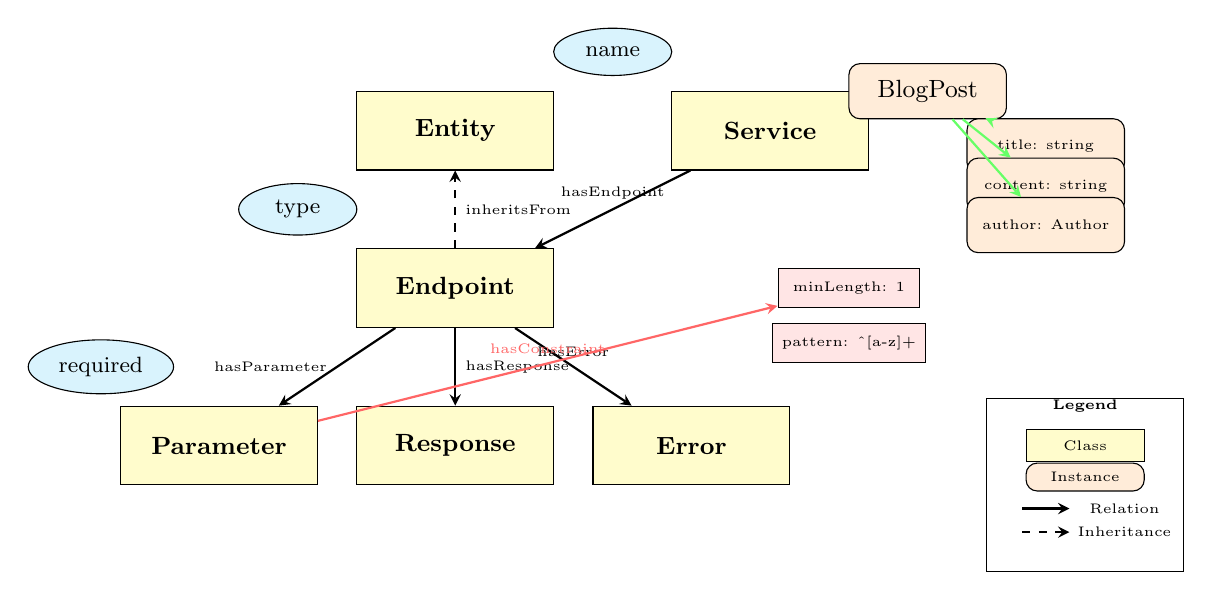
\begin{tikzpicture}[
    class/.style={rectangle, draw, fill=yellow!20, minimum width=2.5cm, minimum height=1cm, font=\small\bfseries},
    instance/.style={rectangle, draw, fill=orange!15, rounded corners, minimum width=2cm, minimum height=0.7cm, font=\small},
    property/.style={ellipse, draw, fill=cyan!15, minimum width=1.5cm, minimum height=0.6cm, font=\footnotesize},
    relation/.style={->, >=stealth, thick},
    inheritance/.style={->, >=stealth, thick, dashed},
    constraint/.style={rectangle, draw, fill=red!10, minimum width=1.8cm, minimum height=0.5cm, font=\tiny}
]

% Core classes
\node[class] (entity) at (0,4) {Entity};
\node[class] (service) at (4,4) {Service};
\node[class] (endpoint) at (0,2) {Endpoint};
\node[class] (parameter) at (-3,0) {Parameter};
\node[class] (response) at (0,0) {Response};
\node[class] (error) at (3,0) {Error};

% Properties
\node[property] (name) at (2,5) {name};
\node[property] (type) at (-2,3) {type};
\node[property] (required) at (-4.5,1) {required};

% Relationships
\draw[relation] (service) -- node[above, font=\tiny] {hasEndpoint} (endpoint);
\draw[relation] (endpoint) -- node[left, font=\tiny] {hasParameter} (parameter);
\draw[relation] (endpoint) -- node[right, font=\tiny] {hasResponse} (response);
\draw[relation] (endpoint) -- node[above, font=\tiny] {hasError} (error);
\draw[inheritance] (endpoint) -- node[right, font=\tiny] {inheritsFrom} (entity);

% Constraints
\node[constraint] (c1) at (5,2) {minLength: 1};
\node[constraint] (c2) at (5,1.3) {pattern: \^{}[a-z]+};
\draw[relation, color=red!60] (parameter) -- node[above, font=\tiny] {hasConstraint} (c1);

% Example instances
\node[instance] (blogpost) at (6,4.5) {BlogPost};
\node[instance, font=\tiny] (title) at (7.5,3.8) {title: string};
\node[instance, font=\tiny] (content) at (7.5,3.3) {content: string};
\node[instance, font=\tiny] (author) at (7.5,2.8) {author: Author};

\draw[relation, color=green!60] (blogpost) -- (title);
\draw[relation, color=green!60] (blogpost) -- (content);
\draw[relation, color=green!60] (blogpost) -- (author);

% Legend
\node[draw, rectangle, fill=white, minimum width=2.5cm, minimum height=2.2cm] at (8,-0.5) {};
\node[font=\tiny\bfseries] at (8,0.5) {Legend};
\node[class, minimum width=1.5cm, minimum height=0.4cm, font=\tiny] at (8,0) {Class};
\node[instance, minimum width=1.5cm, minimum height=0.3cm, font=\tiny] at (8,-0.4) {Instance};
\draw[relation] (7.2,-0.8) -- (7.8,-0.8);
\node[font=\tiny] at (8.5,-0.8) {Relation};
\draw[inheritance] (7.2,-1.1) -- (7.8,-1.1);
\node[font=\tiny] at (8.5,-1.1) {Inheritance};

\end{tikzpicture}
\caption{RDF Ontology Structure for API Contract Generation. The semantic model defines core classes (Entity, Service, Endpoint) and their relationships, enabling formal specification of API contracts with constraints and type information. Example instance shown for BlogPost entity.}
\label{fig:rdf-ontology}
\end{figure}

%   etc.
%
% Or compile this file directly to preview all diagrams

\documentclass[11pt]{article}
\usepackage[margin=1in]{geometry}
\usepackage{tikz}
\usetikzlibrary{shapes.geometric, arrows, positioning, shapes.multipart, shapes.symbols}

\begin{document}

\title{Ontology-Driven Code Generation:\\Architectural Diagrams}
\author{PhD Thesis Supporting Materials}
\date{\today}
\maketitle

\tableofcontents
\newpage

\section{System Architecture Overview}
\begin{figure}[h]
\centering
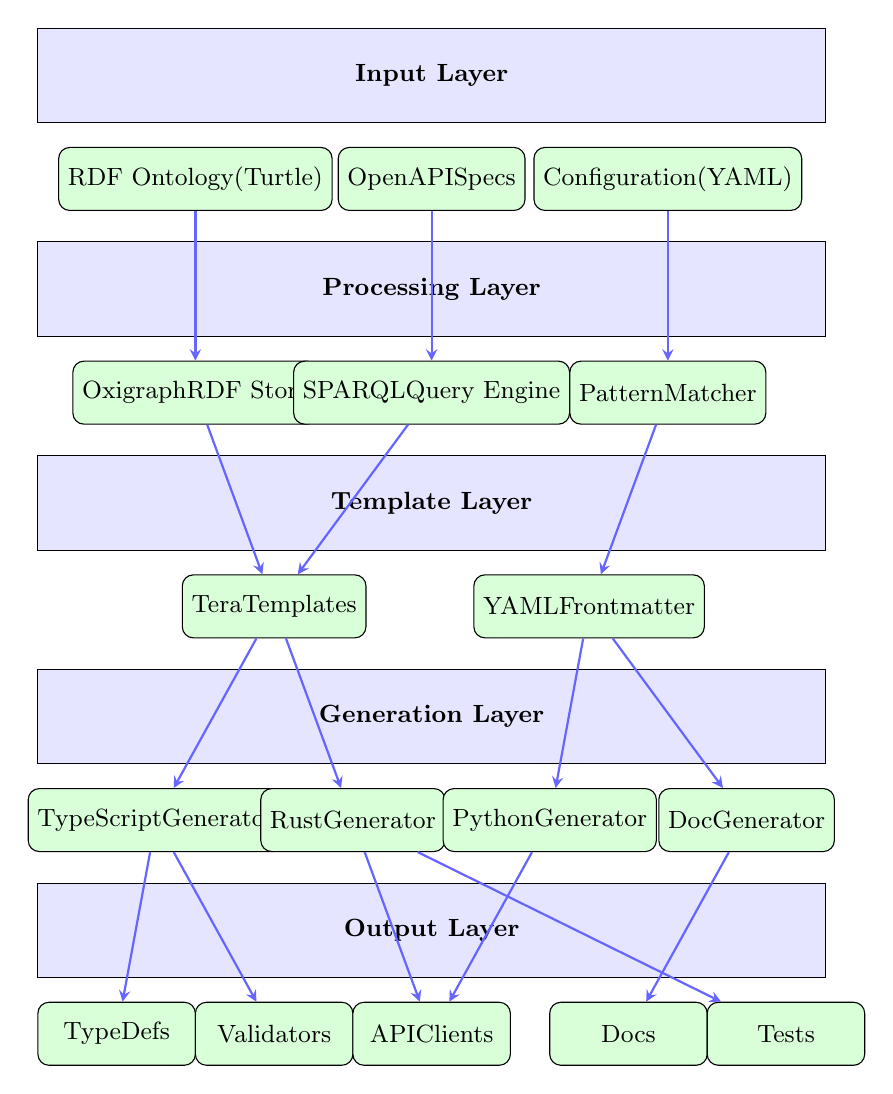
\begin{tikzpicture}[
    layer/.style={rectangle, draw, fill=blue!10, minimum width=10cm, minimum height=1.2cm, font=\small\bfseries},
    component/.style={rectangle, draw, fill=green!15, rounded corners, minimum width=2cm, minimum height=0.8cm, font=\small},
    arrow/.style={->, >=stealth, thick, color=blue!60},
    node distance=0.3cm
]

% Layer 1: Input Layer
\node[layer] (input) at (0,0) {Input Layer};
\node[component, below=of input, xshift=-3cm] (rdf) {RDF Ontology\\(Turtle)};
\node[component, below=of input] (openapi) {OpenAPI\\Specs};
\node[component, below=of input, xshift=3cm] (config) {Configuration\\(YAML)};

% Layer 2: Processing Layer
\node[layer, below=1.5cm of input] (processing) {Processing Layer};
\node[component, below=of processing, xshift=-3cm] (oxigraph) {Oxigraph\\RDF Store};
\node[component, below=of processing] (sparql) {SPARQL\\Query Engine};
\node[component, below=of processing, xshift=3cm] (matcher) {Pattern\\Matcher};

% Layer 3: Template Layer
\node[layer, below=1.5cm of processing] (template) {Template Layer};
\node[component, below=of template, xshift=-2cm] (tera) {Tera\\Templates};
\node[component, below=of template, xshift=2cm] (frontmatter) {YAML\\Frontmatter};

% Layer 4: Generation Layer
\node[layer, below=1.5cm of template] (generation) {Generation Layer};
\node[component, below=of generation, xshift=-3.5cm] (tsgen) {TypeScript\\Generator};
\node[component, below=of generation, xshift=-1cm] (rustgen) {Rust\\Generator};
\node[component, below=of generation, xshift=1.5cm] (pygen) {Python\\Generator};
\node[component, below=of generation, xshift=4cm] (docgen) {Doc\\Generator};

% Layer 5: Output Layer
\node[layer, below=1.5cm of generation] (output) {Output Layer};
\node[component, below=of output, xshift=-4cm] (types) {Type\\Defs};
\node[component, below=of output, xshift=-2cm] (validators) {Validators};
\node[component, below=of output, xshift=0cm] (clients) {API\\Clients};
\node[component, below=of output, xshift=2.5cm] (docs) {Docs};
\node[component, below=of output, xshift=4.5cm] (tests) {Tests};

% Data flow arrows
\draw[arrow] (rdf) -- (oxigraph);
\draw[arrow] (openapi) -- (sparql);
\draw[arrow] (config) -- (matcher);

\draw[arrow] (oxigraph) -- (tera);
\draw[arrow] (sparql) -- (tera);
\draw[arrow] (matcher) -- (frontmatter);

\draw[arrow] (tera) -- (tsgen);
\draw[arrow] (tera) -- (rustgen);
\draw[arrow] (frontmatter) -- (pygen);
\draw[arrow] (frontmatter) -- (docgen);

\draw[arrow] (tsgen) -- (types);
\draw[arrow] (tsgen) -- (validators);
\draw[arrow] (rustgen) -- (clients);
\draw[arrow] (pygen) -- (clients);
\draw[arrow] (docgen) -- (docs);
\draw[arrow] (rustgen) -- (tests);

\end{tikzpicture}
\caption{System Architecture Overview of the ggen Framework. The architecture follows a layered design with clear separation between input specification, semantic processing, template-based transformation, language-specific generation, and artifact output.}
\label{fig:system-architecture}
\end{figure}


\newpage
\section{RDF Ontology Structure}
\begin{figure}[h]
\centering
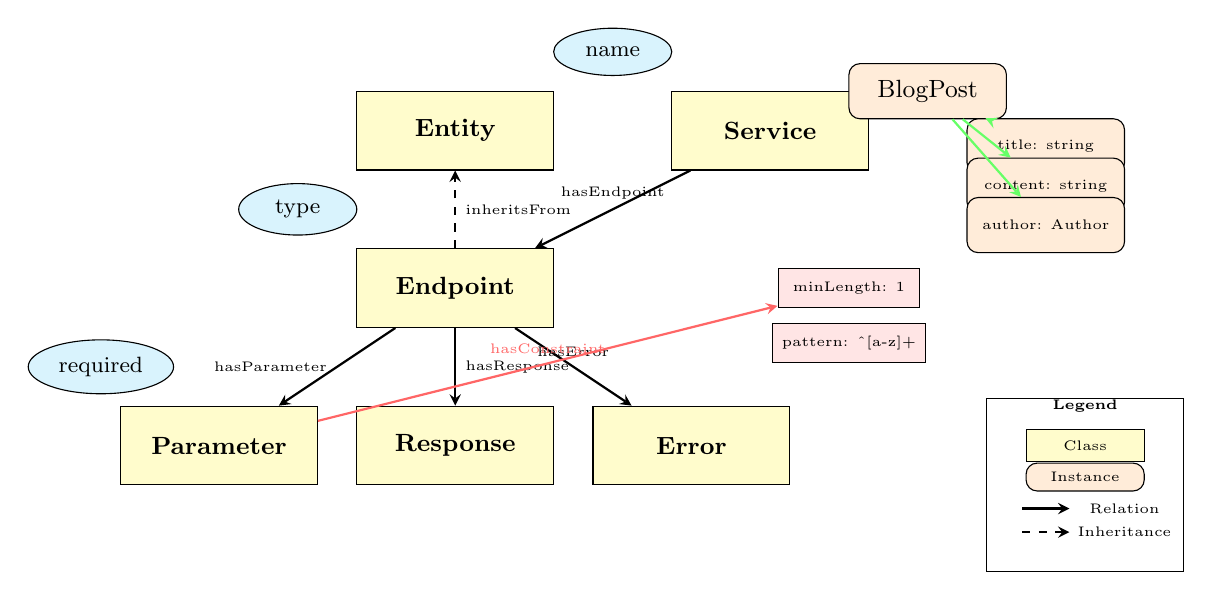
\begin{tikzpicture}[
    class/.style={rectangle, draw, fill=yellow!20, minimum width=2.5cm, minimum height=1cm, font=\small\bfseries},
    instance/.style={rectangle, draw, fill=orange!15, rounded corners, minimum width=2cm, minimum height=0.7cm, font=\small},
    property/.style={ellipse, draw, fill=cyan!15, minimum width=1.5cm, minimum height=0.6cm, font=\footnotesize},
    relation/.style={->, >=stealth, thick},
    inheritance/.style={->, >=stealth, thick, dashed},
    constraint/.style={rectangle, draw, fill=red!10, minimum width=1.8cm, minimum height=0.5cm, font=\tiny}
]

% Core classes
\node[class] (entity) at (0,4) {Entity};
\node[class] (service) at (4,4) {Service};
\node[class] (endpoint) at (0,2) {Endpoint};
\node[class] (parameter) at (-3,0) {Parameter};
\node[class] (response) at (0,0) {Response};
\node[class] (error) at (3,0) {Error};

% Properties
\node[property] (name) at (2,5) {name};
\node[property] (type) at (-2,3) {type};
\node[property] (required) at (-4.5,1) {required};

% Relationships
\draw[relation] (service) -- node[above, font=\tiny] {hasEndpoint} (endpoint);
\draw[relation] (endpoint) -- node[left, font=\tiny] {hasParameter} (parameter);
\draw[relation] (endpoint) -- node[right, font=\tiny] {hasResponse} (response);
\draw[relation] (endpoint) -- node[above, font=\tiny] {hasError} (error);
\draw[inheritance] (endpoint) -- node[right, font=\tiny] {inheritsFrom} (entity);

% Constraints
\node[constraint] (c1) at (5,2) {minLength: 1};
\node[constraint] (c2) at (5,1.3) {pattern: \^{}[a-z]+};
\draw[relation, color=red!60] (parameter) -- node[above, font=\tiny] {hasConstraint} (c1);

% Example instances
\node[instance] (blogpost) at (6,4.5) {BlogPost};
\node[instance, font=\tiny] (title) at (7.5,3.8) {title: string};
\node[instance, font=\tiny] (content) at (7.5,3.3) {content: string};
\node[instance, font=\tiny] (author) at (7.5,2.8) {author: Author};

\draw[relation, color=green!60] (blogpost) -- (title);
\draw[relation, color=green!60] (blogpost) -- (content);
\draw[relation, color=green!60] (blogpost) -- (author);

% Legend
\node[draw, rectangle, fill=white, minimum width=2.5cm, minimum height=2.2cm] at (8,-0.5) {};
\node[font=\tiny\bfseries] at (8,0.5) {Legend};
\node[class, minimum width=1.5cm, minimum height=0.4cm, font=\tiny] at (8,0) {Class};
\node[instance, minimum width=1.5cm, minimum height=0.3cm, font=\tiny] at (8,-0.4) {Instance};
\draw[relation] (7.2,-0.8) -- (7.8,-0.8);
\node[font=\tiny] at (8.5,-0.8) {Relation};
\draw[inheritance] (7.2,-1.1) -- (7.8,-1.1);
\node[font=\tiny] at (8.5,-1.1) {Inheritance};

\end{tikzpicture}
\caption{RDF Ontology Structure for API Contract Generation. The semantic model defines core classes (Entity, Service, Endpoint) and their relationships, enabling formal specification of API contracts with constraints and type information. Example instance shown for BlogPost entity.}
\label{fig:rdf-ontology}
\end{figure}


\newpage
\section{Generation Pipeline Flow}
\begin{figure}[h]
\centering
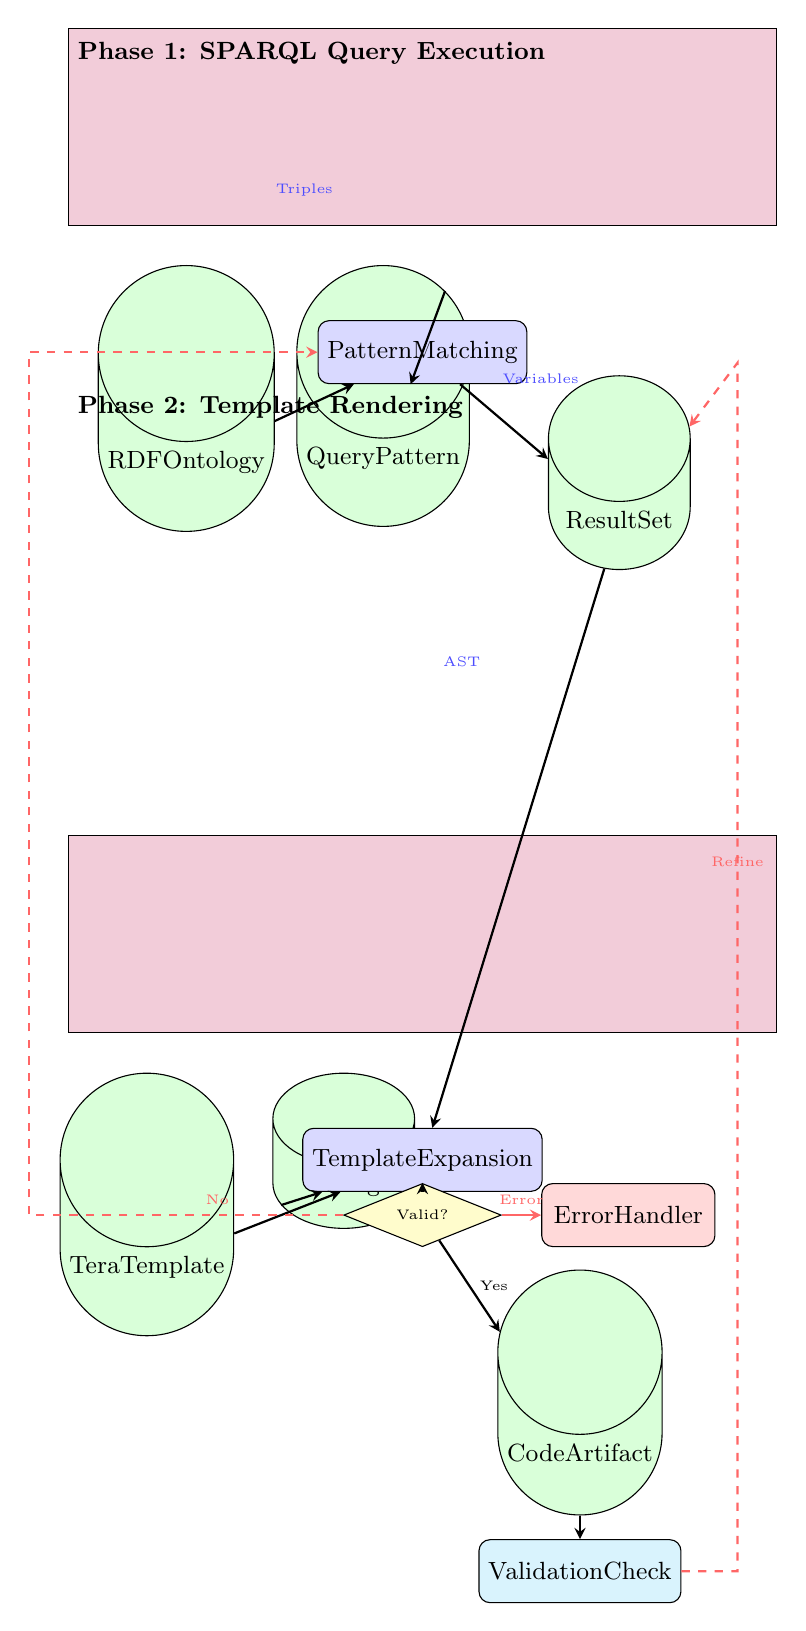
\begin{tikzpicture}[
    phase/.style={rectangle, draw, fill=purple!20, minimum width=9cm, minimum height=2.5cm, font=\bfseries},
    process/.style={rectangle, draw, fill=blue!15, rounded corners, minimum width=2.2cm, minimum height=0.8cm, font=\small},
    data/.style={cylinder, draw, fill=green!15, shape border rotate=90, minimum width=1.8cm, minimum height=0.7cm, font=\small},
    decision/.style={diamond, draw, fill=yellow!20, aspect=2, minimum width=2cm, font=\tiny},
    arrow/.style={->, >=stealth, thick},
    feedback/.style={->, >=stealth, thick, dashed, color=red!60},
    node distance=0.3cm
]

% Phase 1: SPARQL Query Execution
\node[phase] (phase1) at (0,4) {};
\node[font=\small\bfseries, anchor=north west] at (-4.5,5.2) {Phase 1: SPARQL Query Execution};

\node[data, below=0.5cm of phase1, xshift=-3cm] (ontology) {RDF\\Ontology};
\node[data, below=0.5cm of phase1, xshift=-0.5cm] (query) {Query\\Pattern};
\node[process, below=1.2cm of phase1] (matcher) {Pattern\\Matching};
\node[data, below=1.9cm of phase1, xshift=2.5cm] (resultset) {Result\\Set};

\draw[arrow] (ontology) -- (matcher);
\draw[arrow] (query) -- (matcher);
\draw[arrow] (matcher) -- (resultset);

% Phase 2: Template Rendering
\node[phase, below=3.5cm of phase1] (phase2) at (0,-1.5) {};
\node[font=\small\bfseries, anchor=north west] at (-4.5,0.7) {Phase 2: Template Rendering};

\node[data, below=0.5cm of phase2, xshift=-3.5cm] (template) {Tera\\Template};
\node[data, below=0.5cm of phase2, xshift=-1cm] (config) {Config};
\node[process, below=1.2cm of phase2] (renderer) {Template\\Expansion};
\node[decision, below=1.9cm of phase2] (validate) {Valid?};
\node[data, below=3cm of phase2, xshift=2cm] (artifact) {Code\\Artifact};

\draw[arrow] (resultset) -- (renderer);
\draw[arrow] (template) -- (renderer);
\draw[arrow] (config) -- (renderer);
\draw[arrow] (renderer) -- (validate);
\draw[arrow] (validate) -- node[right, font=\tiny] {Yes} (artifact);
\draw[feedback] (validate) -| node[above, font=\tiny, pos=0.2] {No} (-5,-2) |- (matcher);

% Error handling path
\node[process, fill=red!15, right=0.5cm of validate] (error) {Error\\Handler};
\draw[arrow, color=red!60] (validate) -- node[above, font=\tiny] {Error} (error);

% Feedback loop for validation
\node[process, fill=cyan!15, below=0.3cm of artifact] (validation) {Validation\\Check};
\draw[arrow] (artifact) -- (validation);
\draw[feedback] (validation) -| node[below, font=\tiny, pos=0.8] {Refine} (4,1) -- (resultset);

% Labels for data flow
\node[font=\tiny, color=blue!70] at (-1.5,3.2) {Triples};
\node[font=\tiny, color=blue!70] at (1.5,0.8) {Variables};
\node[font=\tiny, color=blue!70] at (0.5,-2.8) {AST};

\end{tikzpicture}
\caption{Generation Pipeline Flow showing the two-phase generation process. Phase 1 executes SPARQL queries against the RDF ontology to extract relevant data. Phase 2 renders Tera templates with the query results and configuration, producing validated code artifacts. Feedback loops enable iterative refinement and error handling.}
\label{fig:generation-pipeline}
\end{figure}


\newpage
\section{Type Guard Composition}
\begin{figure}[h]
\centering
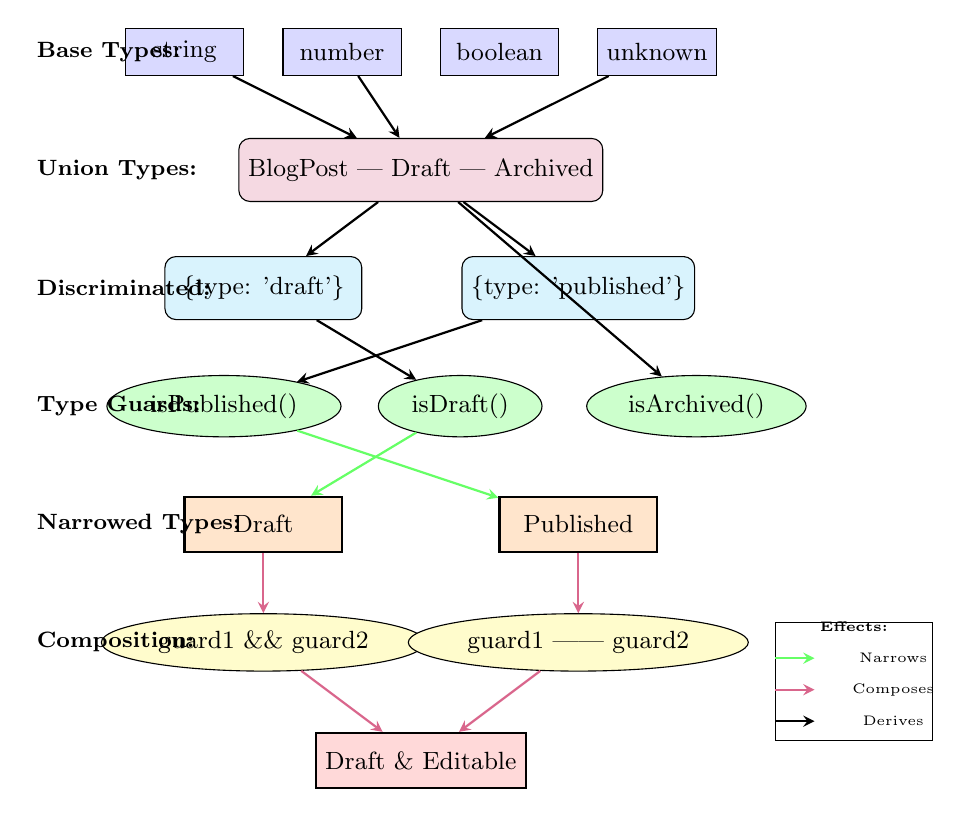
\begin{tikzpicture}[
    basetype/.style={rectangle, draw, fill=blue!15, minimum width=1.5cm, minimum height=0.6cm, font=\small},
    uniontype/.style={rectangle, draw, fill=purple!15, rounded corners, minimum width=2.5cm, minimum height=0.8cm, font=\small},
    guard/.style={ellipse, draw, fill=green!20, minimum width=2cm, minimum height=0.7cm, font=\small},
    narrowed/.style={rectangle, draw, fill=orange!20, thick, minimum width=2cm, minimum height=0.7cm, font=\small},
    arrow/.style={->, >=stealth, thick},
    composition/.style={->, >=stealth, thick, color=purple!60},
    node distance=0.4cm
]

% Base types layer
\node[basetype] (string) at (-3,5) {string};
\node[basetype] (number) at (-1,5) {number};
\node[basetype] (boolean) at (1,5) {boolean};
\node[basetype] (unknown) at (3,5) {unknown};

\node[font=\footnotesize\bfseries, anchor=west] at (-5,5) {Base Types:};

% Union type layer
\node[uniontype] (union1) at (0,3.5) {BlogPost | Draft | Archived};
\node[font=\footnotesize\bfseries, anchor=west] at (-5,3.5) {Union Types:};

\draw[arrow] (string) -- (union1);
\draw[arrow] (number) -- (union1);
\draw[arrow] (unknown) -- (union1);

% Discriminated union layer
\node[uniontype, fill=cyan!15] (disc1) at (-2,2) {\{type: 'draft'\}};
\node[uniontype, fill=cyan!15] (disc2) at (2,2) {\{type: 'published'\}};
\node[font=\footnotesize\bfseries, anchor=west] at (-5,2) {Discriminated:};

\draw[arrow] (union1) -- (disc1);
\draw[arrow] (union1) -- (disc2);

% Type guard functions layer
\node[guard] (ispub) at (-2.5,0.5) {isPublished()};
\node[guard] (isdraft) at (0.5,0.5) {isDraft()};
\node[guard] (isarch) at (3.5,0.5) {isArchived()};

\node[font=\footnotesize\bfseries, anchor=west] at (-5,0.5) {Type Guards:};

\draw[arrow] (disc1) -- (isdraft);
\draw[arrow] (disc2) -- (ispub);
\draw[arrow] (union1) -- (isarch);

% Narrowing effect
\node[narrowed] (narrow1) at (-2,-1) {Draft};
\node[narrowed] (narrow2) at (2,-1) {Published};

\node[font=\footnotesize\bfseries, anchor=west] at (-5,-1) {Narrowed Types:};

\draw[arrow, color=green!60, thick] (isdraft) -- (narrow1);
\draw[arrow, color=green!60, thick] (ispub) -- (narrow2);

% Composition operators
\node[guard, fill=yellow!20] (and) at (-2,-2.5) {guard1 \&\& guard2};
\node[guard, fill=yellow!20] (or) at (2,-2.5) {guard1 || guard2};

\node[font=\footnotesize\bfseries, anchor=west] at (-5,-2.5) {Composition:};

\draw[composition] (narrow1) -- (and);
\draw[composition] (narrow2) -- (or);

\node[narrowed, fill=red!15] (composed) at (0,-4) {Draft \& Editable};
\draw[arrow, color=purple!60, thick] (and) -- (composed);
\draw[arrow, color=purple!60, thick] (or) -- (composed);

% Legend
\node[draw, rectangle, fill=white, minimum width=2cm, minimum height=1.5cm] at (5.5,-3) {};
\node[font=\tiny\bfseries] at (5.5,-2.3) {Effects:};
\draw[arrow, color=green!60, thick] (4.5,-2.7) -- (5,-2.7);
\node[font=\tiny] at (6,-2.7) {Narrows};
\draw[composition] (4.5,-3.1) -- (5,-3.1);
\node[font=\tiny] at (6,-3.1) {Composes};
\draw[arrow] (4.5,-3.5) -- (5,-3.5);
\node[font=\tiny] at (6,-3.5) {Derives};

\end{tikzpicture}
\caption{Type Guard Composition for Type Narrowing. Base types combine into union types, which can be discriminated using type guards. Guards compose with logical operators (\&\& and ||) to enable precise type narrowing, allowing TypeScript to infer more specific types within conditional branches.}
\label{fig:type-guard-composition}
\end{figure}


\newpage
\section{Multi-Artifact Consistency}
\begin{figure}[h]
\centering
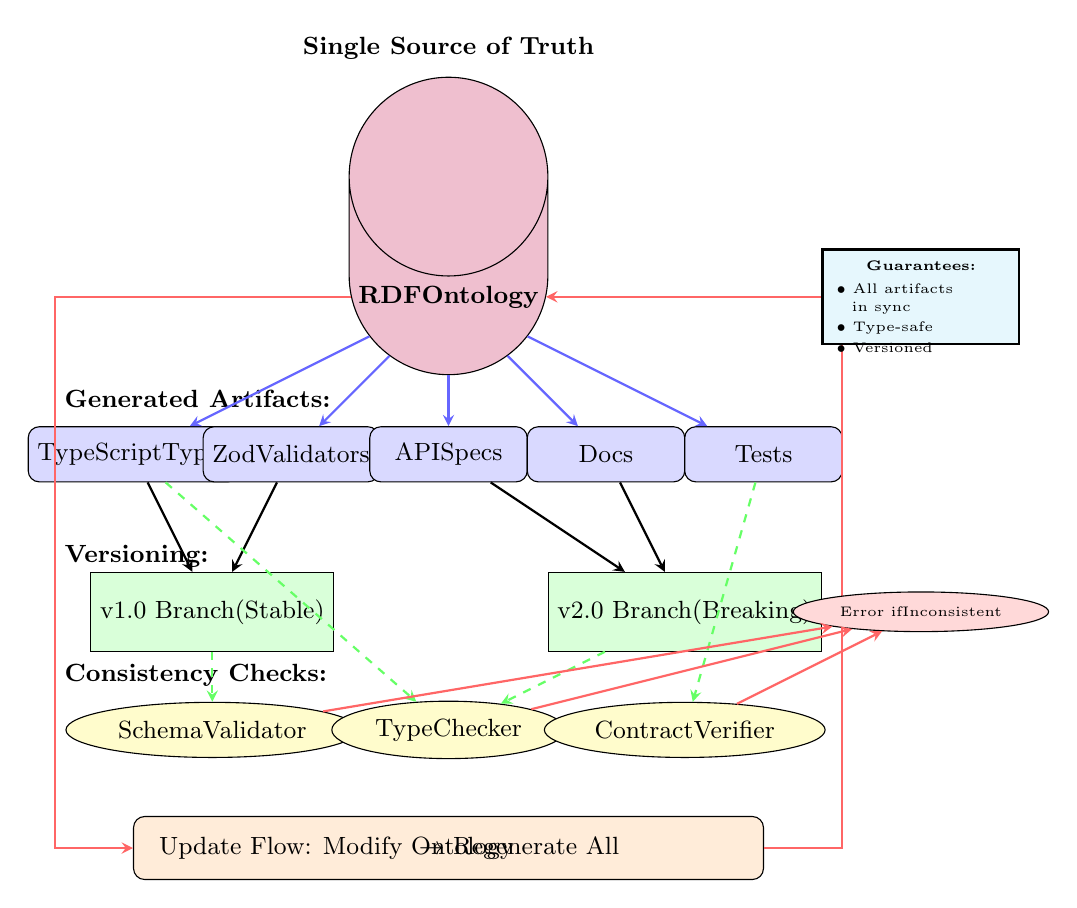
\begin{tikzpicture}[
    source/.style={cylinder, draw, fill=purple!25, shape border rotate=90, minimum width=2.5cm, minimum height=1cm, font=\small\bfseries},
    artifact/.style={rectangle, draw, fill=blue!15, rounded corners, minimum width=2cm, minimum height=0.7cm, font=\small},
    version/.style={rectangle, draw, fill=green!15, minimum width=2.5cm, minimum height=1cm, font=\small},
    validation/.style={ellipse, draw, fill=yellow!20, minimum width=2.2cm, minimum height=0.7cm, font=\small},
    arrow/.style={->, >=stealth, thick},
    generate/.style={->, >=stealth, thick, color=blue!60},
    validate/.style={->, >=stealth, thick, color=green!60, dashed},
    update/.style={->, >=stealth, thick, color=red!60},
    node distance=0.4cm
]

% Single source of truth
\node[source] (ontology) at (0,4.5) {RDF\\Ontology};
\node[font=\small\bfseries, above=0.1cm of ontology] {Single Source of Truth};

% Generated artifacts
\node[artifact] (types) at (-4,2.5) {TypeScript\\Types};
\node[artifact] (zod) at (-2,2.5) {Zod\\Validators};
\node[artifact] (api) at (0,2.5) {API\\Specs};
\node[artifact] (docs) at (2,2.5) {Docs};
\node[artifact] (tests) at (4,2.5) {Tests};

\node[font=\small\bfseries, anchor=west] at (-5,3.2) {Generated Artifacts:};

% Generation arrows
\draw[generate] (ontology) -- (types);
\draw[generate] (ontology) -- (zod);
\draw[generate] (ontology) -- (api);
\draw[generate] (ontology) -- (docs);
\draw[generate] (ontology) -- (tests);

% Versioning layer
\node[version] (v1) at (-3,0.5) {v1.0 Branch\\(Stable)};
\node[version] (v2) at (3,0.5) {v2.0 Branch\\(Breaking)};

\node[font=\small\bfseries, anchor=west] at (-5,1.2) {Versioning:};

\draw[arrow] (types) -- (v1);
\draw[arrow] (zod) -- (v1);
\draw[arrow] (api) -- (v2);
\draw[arrow] (docs) -- (v2);

% Consistency checking
\node[validation] (check1) at (-3,-1) {Schema\\Validator};
\node[validation] (check2) at (0,-1) {Type\\Checker};
\node[validation] (check3) at (3,-1) {Contract\\Verifier};

\node[font=\small\bfseries, anchor=west] at (-5,-0.3) {Consistency Checks:};

\draw[validate] (v1) -- (check1);
\draw[validate] (v2) -- (check2);
\draw[validate] (types) -- (check2);
\draw[validate] (tests) -- (check3);

% Update flow
\node[rectangle, draw, fill=orange!15, rounded corners, minimum width=8cm, minimum height=0.8cm] (update) at (0,-2.5) {};
\node[font=\small, anchor=west] at (-3.8,-2.5) {Update Flow: Modify Ontology};
\node[font=\small, anchor=west] at (-0.5,-2.5) {$\rightarrow$ Regenerate All};

\draw[update] (ontology) -| (-5,2) |- (update);
\draw[update] (update) -| (5,2) |- (ontology);

% Consistency guarantee box
\node[rectangle, draw, thick, fill=cyan!10, minimum width=2.5cm, minimum height=1.2cm] (guarantee) at (6,4.5) {};
\node[font=\tiny\bfseries] at (6,4.9) {Guarantees:};
\node[font=\tiny, align=left, anchor=west] at (4.8,4.6) {$\bullet$ All artifacts};
\node[font=\tiny, align=left, anchor=west] at (5,4.35) {in sync};
\node[font=\tiny, align=left, anchor=west] at (4.8,4.1) {$\bullet$ Type-safe};
\node[font=\tiny, align=left, anchor=west] at (4.8,3.85) {$\bullet$ Versioned};

% Error detection
\node[validation, fill=red!15, minimum width=1.5cm, minimum height=0.5cm, font=\tiny] (error) at (6,0.5) {Error if\\Inconsistent};
\draw[arrow, color=red!60] (check1) -- (error);
\draw[arrow, color=red!60] (check2) -- (error);
\draw[arrow, color=red!60] (check3) -- (error);

\end{tikzpicture}
\caption{Multi-Artifact Consistency Maintenance. The RDF ontology serves as the single source of truth from which all artifacts (types, validators, APIs, documentation, tests) are generated. Automated consistency checks validate artifacts across versions, and the update flow ensures all artifacts remain synchronized when the ontology changes.}
\label{fig:multi-artifact-consistency}
\end{figure}


\end{document}
